\documentclass[11pt,a4paper]{article}
\usepackage{graphicx}
\DeclareGraphicsExtensions{.pdf, .png, .jpg}
\usepackage{style}

\renewcommand{\thesection}{S\arabic{section}}
\renewcommand{\thefigure}{S\arabic{figure}}
\renewcommand{\thetable}{S\arabic{table}}

\sloppy

\title{The Influence of Temperature on Ozone Production under varying \ce{NO_x} Conditions -- a modelling study: Supplementary Material}
\author[1]{J. Coates}
\author[1]{K. A. Mar}
\author[2]{N. Ojha}
\author[1]{T. M. Butler}
\affil[1]{Institute for Advanced Sustainability Studies, Potsdam, Germany}
\affil[2]{Atmospheric Chemistry Department, Max Planck Institute for Chemistry, Mainz, Germany}

\renewcommand\Authands{ and }

\begin{document}

\maketitle

\section{Allocation of Benelux AVOC emissions to Mechanism Species}
Anthropogenic NMVOC emissions over Benelux specified by the TNO\_MACCIII emission inventory \citep{Kuenen:2014} were translated to MCM~v3.2 emissions (Table~\ref{t:Benelux_MCM_emissions}).
The MCM~v3.2 emissions for each initial species were translated to emissions of mechanism species into CRI~v2, MOZART-4 and RADM2 chemical mechanisms by weighting with the carbon numbers (Tables~\ref{t:CRI_NMVOC_emissions} -- \ref{t:RADM2_NMVOC_emissions}).
The allocation of MCM~v3.2 emissions into CB05 species followed the recommendations of \citet{Yarwood:2005} (Table~\ref{t:CB05_NMVOC_emissions}).
{
    \begin{landscape}%
        \centering%
        \tiny
\begin{longtable}{lllllllllllllll}
    \caption{Speciated TNO\_MACCIII emissions for Benelux AVOC and BVOC emissions (molecules~cm$^{-2}$~s$^{-1}$) mapped to MCM~v3.2 species \citep{Kuenen:2014}.}\\%
	\hline \hline
	\textbf{Type} & \textbf{MCM.Species} & \textbf{SNAP.1} & \textbf{SNAP.2} & \textbf{SNAP.34} & \textbf{SNAP.5} & \textbf{SNAP.6} & \textbf{SNAP.71} & \textbf{SNAP.72} & \textbf{SNAP.73} & \textbf{SNAP.74} & \textbf{SNAP.8} & \textbf{SNAP.9} & \textbf{BVOC} & \textbf{Total}\\
	\endhead
	\hline
	Ethane & C2H6 & 9.85e+08 & 1668300000 & 9.18e+09 &  &  & 9.67e+08 & 2.96e+08 & 63860000 &  & 3.45e+08 & 210200000 &  & 1.3728e+10 \\
	\hline Propane & C3H8 & 2.886e+09 & 1086600000 & 2.573e+09 & 1.041e+11 & 9.72e+08 & 47090000 & 202400000 & 638600000 & 62710000 & 249700000 & 75200000 &  & 1.129e+11 \\ \hline
	\multirow{2}{*}{Butanes} & NC4H10 & 2.127e+09 & 882870000 & 949270000 & 6.11e+11 & 3.61e+09 & 1.048e+09 & 209500000 &  & 1037800000 & 315300000 & 42200000 &  & 6.21e+11 \\
	 & IC4H10 & 258600000 & 309660000 & 232311000 & 1.486e+11 & 163700000 & 489100000 & 97500000 &  & 483900000 & 157900000 & 42200000 &  & 1.509e+11 \\
	\hline \multirow{3}{*}{Pentanes} & NC5H12 & 1.783e+09 & 1014960000 &  & 4.548e+11 &  & 6.27e+08 & 8.4e+07 &  & 521500000 & 118200000 & 14890000 &  & 4.589e+11 \\
	 & IC5H12 & 7.52e+08 & 544340000 &  & 2.718e+11 &  & 1.216e+09 & 163500000 &  & 1011700000 & 225600000 & 14890000 &  & 2.762e+11 \\
	 & NEOP &  &  &  &  &  &  &  &  &  &  & 14890000 &  & 14890000 \\
	\hline \parbox[t]{2mm}{\multirow{14}{*}{\rotatebox[origin=c]{90}{Hexane and Higher Alkanes}}} & NC6H14 & 954100000 & 57390000 & 1.211e+09 & 6.49e+10 & 3.162e+09 & 2.207e+09 & 1.246e+09 &  & 193450000 & 4.26e+08 & 5160000 &  & 7.44e+10 \\
	 & M2PE &  &  & 156600000 & 9.98e+09 & 6.66e+08 &  &  &  &  & 7.08e+08 & 2215000 &  & 1.151e+10 \\
	 & M3PE &  &  & 117100000 & 4.989e+09 & 6.66e+08 &  &  &  &  & 4.26e+08 &  &  & 6.2e+09 \\
	 & NC7H16 & 409520000 & 98740000 & 5.71e+08 & 6.97e+10 & 1.146e+09 & 363500000 & 205300000 &  & 31790000 & 121900000 & 26040000 &  & 7.28e+10 \\
	 & M2HEX &  &  &  &  & 4.3e+08 & 2.83e+08 & 159500000 &  & 24710000 & 182900000 &  &  & 1.08e+09 \\
	 & M3HEX &  &  &  &  & 4.3e+08 & 2.02e+08 & 1.14e+08 &  & 17634000 & 121900000 &  &  & 8.86e+08 \\
	 & M22C4 &  &  &  &  &  &  &  &  &  & 141800000 &  &  & 141800000 \\
	 & M23C4 &  &  &  &  &  &  &  &  &  & 141800000 &  &  & 141800000 \\
	 & NC8H18 &  &  & 235300000 & 5.18e+10 & 125600000 & 319500000 & 179700000 &  & 27890000 & 6.95e+08 & 8900000 &  & 5.33e+10 \\
	 & NC9H20 &  &  & 131200000 &  & 3.02e+09 &  &  &  &  &  & 2969000 &  & 3.148e+09 \\
	 & NC10H22 &  &  & 1.66e+08 &  & 5.85e+09 & 142200000 & 80300000 &  & 12458000 &  & 4460000 &  & 6.25e+09 \\
	 & NC11H24 &  &  & 64600000 &  & 2.387e+09 & 51830000 & 29280000 &  & 4536000 & 78100000 & 1625000 &  & 2.617e+09 \\
	 & NC12H26 &  &  &  &  & 168500000 & 8.45e+08 & 476900000 &  & 74100000 & 71700000 &  &  & 1.637e+09 \\
	 & CHEX &  & 91490000 & 4e+07 &  & 6.82e+08 &  &  &  &  &  & 1506000 &  & 8.15e+08 \\
	\hline Ethene & C2H4 & 212300000 & 3695700000 & 3.368e+10 &  &  & 5.341e+09 & 3.807e+09 & 342500000 &  & 4.62e+09 & 1.9e+08 &  & 5.188e+10 \\ \hline
	Propene & C3H6 & 141700000 & 868200000 & 6.59e+08 &  &  & 1.876e+09 & 634800000 & 151810000 &  & 7.86e+08 & 54500000 &  & 5.18e+09 \\
	\hline \parbox[t]{2mm}{\multirow{11}{*}{\rotatebox[origin=c]{90}{Higher Alkenes}}} & HEX1ENE & 21050000 & 15773000 &  &  &  &  &  &  &  &  & 21810000 &  & 58703000 \\
	 & BUT1ENE &  & 22154000 & 240400000 &  &  &  &  &  &  & 24510000 &  &  & 286604000 \\
	 & MEPROPENE &  &  &  &  &  &  &  &  &  & 12260000 &  &  & 12260000 \\
	 & TBUT2ENE &  &  &  &  &  &  &  &  &  & 12260000 &  &  & 12260000 \\
	 & CBUT2ENE &  &  &  &  &  &  &  &  &  & 12260000 &  &  & 12260000 \\
	 & CPENT2ENE &  & 6961000 &  &  &  &  &  &  &  & 4902000 &  &  & 11861000 \\
	 & TPENT2ENE &  & 6961000 &  &  &  &  &  &  &  & 4902000 &  &  & 11861000 \\
	 & PENT1ENE &  & 6328000 & 6186000 &  &  &  &  &  &  & 19630000 &  &  & 32171000 \\
	 & ME2BUT2ENE &  & 3793000 &  &  &  &  &  &  &  & 9800000 &  &  & 13581000 \\
	 & ME3BUT1ENE &  & 3793000 &  &  &  &  &  &  &  & 9800000 &  &  & 13581000 \\
	 & ME2BUT1ENE &  & 2525500 &  &  &  &  &  &  &  &  &  &  & 2525500 \\
	\hline Ethyne & C2H2 & 2697000 & 1252200000 & 426600000 &  &  & 4.975e+09 & 1.795e+09 & 134690000 & 252500000 & 1.614e+09 & 71500000 &  & 1.051e+10 \\ \hline
	Benzene & BENZENE & 269600000 & 1.006e+09 & 8.3e+08 & 1.621e+10 &  & 1.197e+09 & 228300000 &  & 35380000 & 2.83e+08 & 36540000 &  & 2.014e+10 \\
	\hline Toluene & TOLUENE & 252700000 & 372760000 & 84400000 & 1.375e+10 & 6.8e+09 & 2.708e+09 & 1.45e+08 &  & 30030000 & 193900000 & 24100000 &  & 2.435e+10 \\ \hline
	\multirow{3}{*}{Xylenes} & MXYL & 1.05e+08 & 21179000 & 1669300 & 1.994e+09 & 3.93e+09 & 5.77e+08 & 61040000 &  & 4735000 & 70200000 & 4880000 &  & 6.78e+09 \\
	 & OXYL & 23330000 & 21179000 & 669700 & 1.994e+09 & 9.84e+08 & 5.77e+08 & 61040000 &  & 4735000 & 57100000 & 2924000 &  & 3.717e+09 \\
	 & PXYL &  & 21179000 & 669700 & 1.994e+09 & 9.84e+08 & 432900000 & 45800000 &  & 3551000 & 70200000 & 3909000 &  & 3.556e+09 \\
	\hline \multirow{3}{*}{Trimethylbenzenes} & TM123B & 18550 & 1304500 &  &  & 6.6e+07 & 99200000 &  &  &  & 3330000 & 441000 &  & 170200000 \\
	 & TM124B & 18550 & 1304500 & 56100000 &  & 224600000 & 4.16e+08 &  &  &  & 7760000 & 589000 &  & 7.06e+08 \\
	 & TM135B & 18550 & 1304500 &  &  & 6.6e+07 & 158600000 &  &  &  & 3330000 & 589000 &  & 229900000 \\
	\hline \parbox[t]{2mm}{\multirow{11}{*}{\rotatebox[origin=c]{90}{Other Aromatics}}} & EBENZ & 35100000 &  & 63400000 &  & 179400000 & 430600000 & 341600000 & 119530 &  & 8e+08 & 5250000 &  & 1.856e+09 \\
	 & PBENZ &  &  &  &  & 39600000 & 380600000 & 301500000 & 105570 &  & 128500000 & 2311000 &  & 8.53e+08 \\
	 & IPBENZ &  &  &  &  & 145300000 &  &  &  &  & 128500000 & 2311000 &  & 276300000 \\
	 & PETHTOL &  &  &  &  & 13210000 &  &  &  &  & 257500000 &  &  & 270300000 \\
	 & METHTOL &  &  &  &  & 39600000 &  &  &  &  & 257500000 &  &  & 296300000 \\
	 & OETHTOL &  &  &  &  &  &  &  &  &  & 192800000 &  &  & 192800000 \\
	 & DIET35TOL &  &  &  &  &  & 8.05e+08 & 637600000 & 223800 &  &  &  &  & 1.443e+09 \\
	 & DIME35EB &  &  &  &  & 224700000 & 99300000 & 78700000 & 27540 &  &  &  &  & 4.03e+08 \\
	 & STYRENE &  &  & 64600000 &  & 45700000 & 91500000 & 72500000 & 25440 &  &  &  &  & 275100000 \\
	 & BENZAL &  &  &  &  &  & 153900000 & 121900000 & 42690 &  &  &  &  & 275900000 \\
	 & PHENOL &  &  & 71500000 &  &  &  &  &  &  &  &  &  & 71500000 \\
	\hline Formaldehyde & HCHO & 611400000 & 2195300000 &  &  &  & 1.177e+09 & 1.781e+09 & 85260000 &  & 2.9e+09 & 29490000 &  & 8.77e+09 \\ \hline
	\parbox[t]{2mm}{\multirow{9}{*}{\rotatebox[origin=c]{90}{Other Aldehydes}}} & CH3CHO & 11780000 & 130090000 & 73750000 &  &  & 318400000 & 7.39e+08 & 16383000 &  & 6.8e+08 & 6860000 &  & 1.976e+09 \\
	 & C2H5CHO & 6710000 & 98630000 &  &  &  & 53670000 & 124600000 & 2752000 &  & 257700000 & 5200000 &  & 5.49e+08 \\
	 & C3H7CHO & 38630 & 79420000 &  &  &  &  &  &  &  & 207600000 & 4190000 &  & 292100000 \\
	 & IPRCHO & 38630 & 79420000 &  &  &  &  &  &  &  & 138400000 & 4190000 &  & 222100000 \\
	 & C4H9CHO & 32340 & 66550000 &  &  &  &  &  &  &  &  & 3504000 &  & 70050000 \\
	 & ACR & 49770 & 102260000 &  &  &  & 83300000 & 193800000 & 4282000 &  &  & 5390000 &  & 388800000 \\
	 & MACR & 39730 & 81710000 &  &  &  &  &  &  &  &  & 4310000 &  & 86110000 \\
	 & C4ALDB & 39730 & 81710000 &  &  &  & 44510000 & 103300000 & 2287000 &  &  & 4310000 &  & 236100000 \\
	 & MGLYOX &  &  &  &  &  &  &  &  &  & 138500000 &  &  & 138500000 \\
	\hline Alkadienes and & C4H6 & 67600000 & 771300000 & 4.74e+09 & 2.221e+11 &  & 2.505e+09 & 7.78e+08 & 245800000 & 458800000 & 1.033e+09 & 52800000 &  & 2.332e+11 \\
	Other Alkynes & C5H8 &  &  &  &  &  &  &  &  &  &  &  & 1.435e+10 & 1.435e+10 \\
	\hline \multirow{4}{*}{Organic Acids} & HCOOH & 4660000 & 1201400000 &  &  &  &  &  &  &  & 1.67e+08 & 69400000 &  & 1442400000 \\
	 & CH3CO2H & 3572000 & 9.21e+08 & 167700000 &  &  &  &  &  &  & 1.28e+08 & 53200000 &  & 1.274e+09 \\
	 & PROPACID & 2898000 & 746100000 &  &  &  &  &  &  &  & 1.04e+08 & 43100000 &  & 897100000 \\
	 & ACO2H &  &  & 140400000 &  &  &  &  &  &  &  &  &  & 140400000 \\
	\hline \parbox[t]{2mm}{\multirow{19}{*}{\rotatebox[origin=c]{90}{Alcohols}}} & CH3OH & 140000 &  & 3200000 &  & 6.38e+09 &  &  &  &  & 40419000 & 24020000 &  & 6.45e+09 \\*
	 & C2H5OH & 97400 & 1.687e+09 & 90300000 &  & 6.52e+09 &  &  &  &  & 28082900 & 63300000 &  & 8.39e+09 \\*
	 & NPROPOL & 74600 &  &  &  & 5.31e+08 &  &  &  &  & 21563500 & 7670000 &  & 5.61e+08 \\*
	 & IPROPOL & 74600 &  & 1135000 &  & 8.49e+08 &  &  &  &  & 21563500 &  &  & 8.73e+08 \\*
	 & NBUTOL & 60500 &  &  &  & 5.17e+08 &  &  &  &  & 17451500 &  &  & 5.34e+08 \\
	 & BUT2OL & 60500 &  &  &  & 345400000 &  &  &  &  & 17451500 & 10360000 &  & 3.73e+08 \\
	 & IBUTOL & 60500 &  &  &  & 215300000 &  &  &  &  & 17451500 &  &  & 232800000 \\
	 & TBUTOL & 60500 &  &  &  &  &  &  &  &  & 17451500 &  &  & 17489700 \\
	 & PECOH & 50900 &  &  &  &  &  &  &  &  & 14643300 &  &  & 14775400 \\
	 & IPEAOH & 50900 &  &  &  &  &  &  &  &  & 14643300 &  &  & 14775400 \\
	 & ME3BUOL & 50900 &  &  &  &  &  &  &  &  & 14643300 &  &  & 14775400 \\
	 & IPECOH & 50900 &  &  &  &  &  &  &  &  & 14643300 &  &  & 14775400 \\
	 & IPEBOH & 50900 &  &  &  &  &  &  &  &  & 14643300 &  &  & 14775400 \\
	 & CYHEXOL & 44800 &  &  &  &  &  &  &  &  & 12938100 &  &  & 12966400 \\
	 & MIBKAOH & 38600 &  &  &  & 109900000 &  &  &  &  & 11132900 &  &  & 121100000 \\
	 & ETHGLY & 72300 &  &  &  & 154300000 &  &  &  &  & 20861500 &  &  & 175200000 \\
	 & PROPGLY & 59000 &  &  &  & 307800000 &  &  &  &  & 16950200 &  &  & 324800000 \\
	 & C6H5CH2OH &  &  &  &  & 88500000 &  &  &  &  &  &  &  & 88500000 \\
	 & MBO & 52100 &  &  &  &  &  &  &  &  & 15044300 &  &  & 15077200 \\
	\hline \parbox[t]{2mm}{\multirow{10}{*}{\rotatebox[origin=c]{90}{Ketones}}} & CH3COCH3 & 384100 & 15896000 & 6.38e+08 &  & 6.66e+09 & 35750000 & 229900000 &  &  & 382100000 & 1414000 &  & 7.96e+09 \\
	 & MEK &  & 12828000 &  &  & 3.212e+09 &  &  &  &  &  & 1139000 &  & 3.236e+09 \\
	 & MPRK &  & 10745000 &  &  &  &  &  &  &  &  & 954000 &  & 11705000 \\
	 & DIEK &  & 10745000 &  &  &  &  &  &  &  &  & 954000 &  & 11705000 \\
	 & MIPK &  & 10745000 &  &  &  &  &  &  &  &  & 954000 &  & 11705000 \\
	 & HEX2ONE &  & 9242000 &  &  &  &  &  &  &  &  & 820000 &  & 10062000 \\
	 & HEX3ONE &  & 9242000 &  &  &  &  &  &  &  &  & 820000 &  & 10062000 \\
	 & MIBK &  & 9242000 &  &  & 1.93e+09 &  &  &  &  &  & 820000 &  & 1.94e+09 \\
	 & MTBK &  & 9242000 &  &  &  &  &  &  &  &  & 820000 &  & 10062000 \\
	 & CYHEXONE &  & 9439000 & 34310000 &  & 157500000 &  &  &  &  &  & 837000 &  & 202200000 \\
	\hline \multirow{3}{*}{Terpenes} & APINENE &  &  &  &  &  &  &  &  &  &  & 3050000 & 1.835e+09 & 1.839e+09 \\
	 & BPINENE &  &  &  &  &  &  &  &  &  &  & 3050000 & 1.835e+09 & 1.839e+09 \\
	 & LIMONENE &  &  &  &  & 209500000 &  &  &  &  &  & 4580000 & 1.835e+09 & 2.046e+09 \\
	\hline \parbox[t]{2mm}{\multirow{6}{*}{\rotatebox[origin=c]{90}{Esters}}} & METHACET &  &  & 64470000 &  &  &  &  &  &  &  &  &  & 64470000 \\
	 & ETHACET &  &  & 7386000 &  & 4.44e+09 &  &  &  &  &  &  &  & 4.45e+09 \\
	 & NBUTACET &  &  &  &  & 3.113e+09 &  &  &  &  &  &  &  & 3.113e+09 \\
	 & IPROACET &  &  &  &  & 1.095e+09 &  &  &  &  &  &  &  & 1.095e+09 \\
	 & CH3OCHO &  &  & 7229000 &  &  &  &  &  &  &  &  &  & 7229000 \\
	 & NPROACET &  &  &  &  & 4.1e+08 &  &  &  &  &  & 7950000 &  & 4.18e+08 \\
	\hline \parbox[t]{2mm}{\multirow{10}{*}{\rotatebox[origin=c]{90}{Ethers}}} & CH3OCH3 &  & 61750000 & 253500000 &  & 244300000 &  &  &  &  &  &  &  & 5.59e+08 \\*
	 & DIETETHER &  & 38360000 & 94510000 &  &  &  &  &  &  &  &  &  & 132360000 \\
	 & MTBE &  & 32330000 &  &  &  &  &  &  &  &  &  &  & 32330000 \\
	 & DIIPRETHER &  & 27860000 & 68540000 &  &  &  &  &  &  &  & 19520000 &  & 115960000 \\
	 & ETBE &  & 27860000 &  &  &  &  &  &  &  &  &  &  & 27860000 \\
	 & MO2EOL &  & 37420000 &  &  & 295700000 &  &  &  &  &  &  &  & 3.33e+08 \\
	 & EOX2EOL &  & 31600000 &  &  & 249900000 &  &  &  &  &  &  &  & 281500000 \\
	 & PR2OHMOX &  & 31600000 &  &  & 5e+08 &  &  &  &  &  &  &  & 5.32e+08 \\
	 & BUOX2ETOH &  & 24117000 &  &  & 2.398e+09 &  &  &  &  &  &  &  & 2.422e+09 \\
	 & BOX2PROL &  & 21510000 &  &  &  &  &  &  &  &  &  &  & 21510000 \\
	\hline \parbox[t]{2mm}{\multirow{12}{*}{\rotatebox[origin=c]{90}{Chlorinated Hydrocarbons}}} & CH2CL2 &  &  & 6.74e+08 &  & 1.589e+09 &  &  &  &  &  & 1458000 &  & 2.262e+09 \\
	 & CH3CH2CL &  &  & 5.22e+08 &  &  &  &  &  &  &  &  &  & 5.22e+08 \\
	 & CH3CCL3 &  &  &  &  & 1.113e+09 &  &  &  &  &  & 464000 &  & 1.114e+09 \\
	 & TRICLETH &  &  & 256600000 &  & 2.516e+09 &  &  &  &  &  & 471000 &  & 2.776e+09 \\
	 & CDICLETH &  &  & 173100000 &  &  &  &  &  &  &  & 951000 &  & 174800000 \\
	 & TDICLETH &  &  & 173100000 &  &  &  &  &  &  &  & 634000 &  & 174600000 \\
	 & CH3CL &  &  & 5.34e+08 &  &  &  &  &  &  &  &  &  & 5.34e+08 \\
	 & CCL2CH2 &  &  & 173100000 &  &  &  &  &  &  &  &  &  & 173100000 \\
	 & CHCL2CH3 &  &  &  &  &  &  &  &  &  &  & 715000 &  & 715000 \\
	 & VINCL &  &  & 1.62e+08 &  &  &  &  &  &  &  &  &  & 1.62e+08 \\
	 & TCE &  &  & 40500000 &  & 6.11e+08 &  &  &  &  &  & 927000 &  & 6.53e+08 \\
	 & CHCL3 &  &  & 112800000 &  &  &  &  &  &  &  &  &  & 112800000 \\
	\hline \multicolumn{2}{c}{Total}  & 1.192e+10 & 2.1806e+10 & 6.11e+10 & 2.049e+12 & 8.39e+10 & 3.33e+10 & 1.581e+10 & 1688300000 & 4.285e+09 & 2.059e+10 & 1.333e+09 & 1.9847e+10 & 2.32e+12 \\
	\hline \hline
	\label{t:Benelux_MCM_emissions}
\end{longtable}

    \end{landscape}%
}
\newpage
{
    \centering%
    \footnotesize
\begin{longtable}{lllllll}
	\caption{Benelux AVOC and BVOC emissions, in molecules~cm$^{-2}$~s$^{-1}$, mapped from MCMv3.2 species into corresponding CRIv2 species. Emissions were weighted by the carbon numbers of the respective species.}\\%
	\hline \hline
	\multirow{2}{*}{\textbf{Type}} & \textbf{MCMv3.2} & \textbf{CRIv2} & \multirow{2}{*}{\textbf{Belgium}} & \multirow{2}{*}{\textbf{Netherlands}} & \multirow{2}{*}{\textbf{Luxembourg}} & \multirow{2}{*}{\textbf{Total}} \\
 & \textbf{Species} & \textbf{Species} & & & & \\
	\endhead
	\hline
	Ethane & C2H6 & C2H6 & 4.91E+09 & 8.58E+08 & 7.96E+09 & 1.37E+10 \\
	\hline Propane & C3H8 & C3H8 & 3.35E+10 & 4.00E+10 & 3.94E+10 & 1.13E+11 \\ \hline
	\multirow{2}{*}{Butanes} & NC4H10 & NC4H10 & 1.25E+11 & 3.49E+11 & 1.47E+11 & 6.21E+11 \\
	 & IC4H10 & IC4H10 & 3.03E+10 & 8.50E+10 & 3.56E+10 & 1.51E+11 \\
	\hline \multirow{3}{*}{Pentanes} & NC5H12 & NC5H12 & 8.89E+10 & 2.65E+11 & 1.05E+11 & 4.59E+11 \\
	 & IC5H12 & IC5H12 & 5.33E+10 & 1.60E+11 & 6.29E+10 & 2.76E+11 \\
	 & NEOP & NEOP & 1.11E+07 & 0.00E+00 & 3.79E+06 & 1.49E+07 \\
	\hline \parbox[t]{2mm}{\multirow{14}{*}{\rotatebox[origin=c]{90}{Hexane and Higher Alkanes}}} & NC6H14 & NC6H14 & 1.52E+10 & 4.10E+10 & 1.82E+10 & 7.44E+10 \\
	 & M2PE & M2PE & 2.39E+09 & 6.28E+09 & 2.84E+09 & 1.15E+10 \\
	 & M3PE & M3PE & 1.34E+09 & 3.29E+09 & 1.57E+09 & 6.20E+09 \\
	 & NC7H16 & NC7H16 & 1.45E+10 & 4.12E+10 & 1.71E+10 & 7.28E+10 \\
	 & M2HEX & M2HEX & 2.74E+08 & 4.89E+08 & 3.17E+08 & 1.08E+09 \\
	 & M3HEX & M3HEX & 2.37E+08 & 3.90E+08 & 2.59E+08 & 8.86E+08 \\
	 & M22C4 & M22C4 & 3.47E+07 & 5.29E+07 & 5.42E+07 & 1.42E+08 \\
	 & M23C4 & M23C4 & 3.47E+07 & 5.29E+07 & 5.42E+07 & 1.42E+08 \\
	 & NC8H18 & NC8H18 & 1.04E+10 & 3.06E+10 & 1.23E+10 & 5.33E+10 \\
	 & NC9H20 & NC9H20 & 1.10E+09 & 1.07E+09 & 9.78E+08 & 3.15E+09 \\
	 & NC10H22 & NC10H22 & 2.15E+09 & 2.21E+09 & 1.89E+09 & 6.25E+09 \\
	 & NC11H24 & NC11H24 & 8.95E+08 & 9.26E+08 & 7.96E+08 & 2.62E+09 \\
	 & NC12H26 & NC12H26 & 3.07E+08 & 8.88E+08 & 4.42E+08 & 1.64E+09 \\
	 & CHEX & CHEX & 2.91E+08 & 2.44E+08 & 2.80E+08 & 8.15E+08 \\
	\hline Ethene & C2H4 & C2H4 & 3.66E+10 & 7.03E+09 & 8.25E+09 & 5.19E+10 \\ \hline
	Propene & C3H6 & C3H6 & 1.82E+09 & 1.68E+09 & 1.68E+09 & 5.18E+09 \\
	\hline \parbox[t]{2mm}{\multirow{11}{*}{\rotatebox[origin=c]{90}{Higher Alkenes}}} & HEX1ENE & HEX1ENE & 3.42E+07 & 5.03E+05 & 2.40E+07 & 5.87E+07 \\
	 & BUT1ENE & BUT1ENE & 9.99E+07 & 7.04E+05 & 1.86E+08 & 2.87E+08 \\
	 & MEPROPENE & MEPROPENE & 9.80E+06 & 0.00E+00 & 2.46E+06 & 1.23E+07 \\
	 & TBUT2ENE & TBUT2ENE & 9.80E+06 & 0.00E+00 & 2.46E+06 & 1.23E+07 \\
	 & CBUT2ENE & CBUT2ENE & 9.80E+06 & 0.00E+00 & 2.46E+06 & 1.23E+07 \\
	 & CPENT2ENE & CPENT2ENE & 9.57E+06 & 2.21E+05 & 2.07E+06 & 1.19E+07 \\
	 & TPENT2ENE & TPENT2ENE & 9.57E+06 & 2.21E+05 & 2.07E+06 & 1.19E+07 \\
	 & PENT1ENE & PENT1ENE & 2.68E+07 & 2.01E+05 & 5.17E+06 & 3.22E+07 \\
	 & ME2BUT2ENE & ME2BUT2ENE & 1.09E+07 & 1.21E+05 & 2.56E+06 & 1.36E+07 \\
	 & ME3BUT1ENE & ME3BUT1ENE & 1.09E+07 & 1.21E+05 & 2.56E+06 & 1.36E+07 \\
	 & ME2BUT1ENE & ME2BUT1ENE & 2.05E+06 & 8.05E+04 & 3.95E+05 & 2.53E+06 \\
	\hline Ethyne & C2H2 & C2H2 & 2.78E+09 & 4.51E+09 & 3.22E+09 & 1.05E+10 \\ \hline
	Benzene & BENZENE & BENZENE & 4.52E+09 & 1.06E+10 & 5.02E+09 & 2.01E+10 \\
	\hline Toluene & TOLUENE & TOLUENE & 5.78E+09 & 1.22E+10 & 6.37E+09 & 2.44E+10 \\ \hline
	\multirow{3}{*}{Xylenes} & MXYL & MXYL & 1.90E+09 & 3.00E+09 & 1.88E+09 & 6.78E+09 \\
	 & OXYL & OXYL & 8.61E+08 & 1.89E+09 & 9.66E+08 & 3.72E+09 \\
	 & PXYL & PXYL & 8.28E+08 & 1.82E+09 & 9.08E+08 & 3.56E+09 \\
	\hline \multirow{3}{*}{Trimethylbenzenes} & TM123B & TM123B & 4.49E+07 & 7.36E+07 & 5.17E+07 & 1.70E+08 \\
	 & TM124B & TM124B & 1.75E+08 & 2.89E+08 & 2.42E+08 & 7.06E+08 \\
	 & TM135B & TM135B & 5.58E+07 & 1.03E+08 & 7.11E+07 & 2.30E+08 \\
	\hline \parbox[t]{2mm}{\multirow{11}{*}{\rotatebox[origin=c]{90}{Other Aromatics}}} & EBENZ & EBENZ & 3.99E+08 & 8.28E+08 & 6.29E+08 & 1.86E+09 \\
	 & PBENZ & PBENZ & 1.59E+08 & 4.63E+08 & 2.31E+08 & 8.53E+08 \\
	 & IPBENZ & IPBENZ & 7.88E+07 & 1.04E+08 & 9.35E+07 & 2.76E+08 \\
	 & PETHTOL & PETHTOL & 6.03E+07 & 1.05E+08 & 1.05E+08 & 2.70E+08 \\
	 & METHTOL & METHTOL & 6.93E+07 & 1.14E+08 & 1.13E+08 & 2.96E+08 \\
	 & OETHTOL & OETHTOL & 4.19E+07 & 7.47E+07 & 7.62E+07 & 1.93E+08 \\
	 & DIET35TOL & DIET35TOL & 2.45E+08 & 8.42E+08 & 3.56E+08 & 1.44E+09 \\
	 & DIME35EB & DIME35EB & 1.06E+08 & 1.88E+08 & 1.09E+08 & 4.03E+08 \\
	 & STYRENE & STYRENE & 6.01E+07 & 1.13E+08 & 1.02E+08 & 2.75E+08 \\
	 & BENZAL & BENZAL & 4.68E+07 & 1.61E+08 & 6.81E+07 & 2.76E+08 \\
	 & PHENOL & AROH14 & 1.86E+07 & 0.00E+00 & 5.29E+07 & 7.15E+07 \\
	\hline Formaldehyde & HCHO & HCHO & 2.35E+09 & 3.04E+09 & 3.38E+09 & 8.77E+09 \\ \hline
	\parbox[t]{2mm}{\multirow{9}{*}{\rotatebox[origin=c]{90}{Other Aldehydes}}} & CH3CHO & CH3CHO & 5.53E+08 & 8.88E+08 & 5.35E+08 & 1.98E+09 \\
	 & C2H5CHO & C2H5CHO & 1.78E+08 & 1.97E+08 & 1.74E+08 & 5.49E+08 \\
	 & C3H7CHO & C3H7CHO & 1.19E+08 & 6.71E+07 & 1.06E+08 & 2.92E+08 \\
	 & IPRCHO & IPRCHO & 9.60E+07 & 4.57E+07 & 8.04E+07 & 2.22E+08 \\
	 & C4H9CHO & C4H9CHO & 4.25E+07 & 2.45E+06 & 2.51E+07 & 7.01E+07 \\
	 & ACR & UCARB10 & 8.33E+07 & 1.35E+08 & 7.33E+07 & 2.92E+08 \\
	 & MACR & UCARB10 & 5.23E+07 & 3.01E+06 & 3.08E+07 & 8.61E+07 \\
	 & C4ALDB & UCARB10 & 7.67E+07 & 9.70E+07 & 6.24E+07 & 2.36E+08 \\
	 & MGLYOX & CARB6 & 4.52E+07 & 2.85E+07 & 3.36E+07 & 1.07E+08 \\
	\hline Alkadienes and & C4H6 & C4H6 & 4.36E+10 & 1.34E+11 & 5.56E+10 & 2.33E+11 \\
	Other Alkynes & C5H8 & C5H8 & 3.35E+09 & 1.10E+10 & 0.00E+00 & 1.44E+10 \\
	\hline \multirow{4}{*}{Organic Acids} & HCOOH & HCOOH & 9.28E+08 & 4.04E+07 & 4.74E+08 & 1.44E+09 \\*
	 & CH3CO2H & CH3CO2H & 7.55E+08 & 3.10E+07 & 4.88E+08 & 1.27E+09 \\*
	 & PROPACID & PROPACID & 5.77E+08 & 2.51E+07 & 2.95E+08 & 8.97E+08 \\
	 & ACO2H & PROPACID & 3.64E+07 & 0.00E+00 & 1.04E+08 & 1.40E+08 \\
	\hline \parbox[t]{2mm}{\multirow{19}{*}{\rotatebox[origin=c]{90}{Alcohols}}} & CH3OH & CH3OH & 2.20E+09 & 2.40E+09 & 1.85E+09 & 6.45E+09 \\
	 & C2H5OH & C2H5OH & 3.30E+09 & 2.51E+09 & 2.58E+09 & 8.39E+09 \\
	 & NPROPOL & NPROPOL & 2.06E+08 & 2.00E+08 & 1.55E+08 & 5.61E+08 \\
	 & IPROPOL & IPROPOL & 3.08E+08 & 3.19E+08 & 2.46E+08 & 8.73E+08 \\
	 & NBUTOL & NBUTOL & 1.91E+08 & 1.94E+08 & 1.49E+08 & 5.34E+08 \\
	 & BUT2OL & BUT2OL & 1.41E+08 & 1.30E+08 & 1.02E+08 & 3.73E+08 \\
	 & IBUTOL & IBUTOL & 8.97E+07 & 8.09E+07 & 6.22E+07 & 2.33E+08 \\
	 & TBUTOL & TBUTOL & 1.74E+07 & 0.00E+00 & 8.97E+04 & 1.75E+07 \\
	 & PECOH & PECOH & 1.47E+07 & 0.00E+00 & 7.54E+04 & 1.48E+07 \\
	 & IPEAOH & IPEAOH & 1.47E+07 & 0.00E+00 & 7.54E+04 & 1.48E+07 \\
	 & ME3BUOL & ME3BUOL & 1.47E+07 & 0.00E+00 & 7.54E+04 & 1.48E+07 \\
	 & IPECOH & IPECOH & 1.47E+07 & 0.00E+00 & 7.54E+04 & 1.48E+07 \\
	 & IPEBOH & IPEBOH & 1.47E+07 & 0.00E+00 & 7.54E+04 & 1.48E+07 \\
	 & CYHEXOL & CYHEXOL & 1.29E+07 & 0.00E+00 & 6.64E+04 & 1.30E+07 \\
	 & MIBKAOH & MIBKAOH & 4.80E+07 & 4.13E+07 & 3.18E+07 & 1.21E+08 \\
	 & ETHGLY & ETHGLY & 7.26E+07 & 5.80E+07 & 4.46E+07 & 1.75E+08 \\
	 & PROPGLY & PROPGLY & 1.20E+08 & 1.16E+08 & 8.88E+07 & 3.25E+08 \\
	 & C6H5CH2OH & BENZAL & 2.31E+07 & 2.59E+07 & 1.99E+07 & 6.89E+07 \\
	 & MBO & PENT1ENE & 1.50E+07 & 0.00E+00 & 7.72E+04 & 1.51E+07 \\
	\hline \parbox[t]{2mm}{\multirow{10}{*}{\rotatebox[origin=c]{90}{Ketones}}} & CH3COCH3 & CH3COCH3 & 2.67E+09 & 2.75E+09 & 2.54E+09 & 7.96E+09 \\
	 & MEK & MEK & 1.11E+09 & 1.20E+09 & 9.26E+08 & 3.24E+09 \\
	 & MPRK & MPRK & 8.03E+06 & 3.75E+05 & 3.30E+06 & 1.17E+07 \\
	 & DIEK & DIEK & 8.03E+06 & 3.75E+05 & 3.30E+06 & 1.17E+07 \\
	 & MIPK & MIPK & 8.03E+06 & 3.75E+05 & 3.30E+06 & 1.17E+07 \\
	 & HEX2ONE & HEX2ONE & 6.90E+06 & 3.22E+05 & 2.84E+06 & 1.01E+07 \\
	 & HEX3ONE & HEX3ONE & 6.90E+06 & 3.22E+05 & 2.84E+06 & 1.01E+07 \\
	 & MIBK & MIBK & 6.67E+08 & 7.17E+08 & 5.56E+08 & 1.94E+09 \\
	 & MTBK & MTBK & 6.90E+06 & 3.22E+05 & 2.84E+06 & 1.01E+07 \\
	 & CYHEXONE & CYHEXONE & 6.99E+07 & 5.89E+07 & 7.34E+07 & 2.02E+08 \\
	\hline \parbox[t]{2mm}{\multirow{10}{*}{\rotatebox[origin=c]{90}{Ethers}}} & CH3OCH3 & CH3OCH3 & 3.59E+08 & 9.30E+07 & 1.07E+08 & 5.59E+08 \\*
	 & DIETETHER & DIETETHER & 1.11E+08 & 1.46E+06 & 1.99E+07 & 1.32E+08 \\*
	 & MTBE & MTBE & 1.76E+07 & 1.23E+06 & 1.35E+07 & 3.23E+07 \\
	 & DIIPRETHER & DIIPRETHER & 9.56E+07 & 1.06E+06 & 1.93E+07 & 1.16E+08 \\
	 & ETBE & ETBE & 1.52E+07 & 1.06E+06 & 1.16E+07 & 2.79E+07 \\
	 & MO2EOL & MO2EOL & 1.21E+08 & 1.11E+08 & 1.01E+08 & 3.33E+08 \\
	 & EOX2EOL & EOX2EOL & 1.02E+08 & 9.39E+07 & 8.56E+07 & 2.82E+08 \\
	 & PR2OHMOX & PR2OHMOX & 1.87E+08 & 1.87E+08 & 1.58E+08 & 5.32E+08 \\
	 & BUOX2ETOH & BUOX2ETOH & 8.27E+08 & 8.90E+08 & 7.05E+08 & 2.42E+09 \\
	 & BOX2PROL & BOX2PROL & 1.17E+07 & 8.20E+05 & 8.99E+06 & 2.15E+07 \\
	\hline \parbox[t]{2mm}{\multirow{12}{*}{\rotatebox[origin=c]{90}{Chlorinated Hydrocarbons}}} & CH2CL2 & C2H2 & 4.17E+08 & 2.04E+08 & 5.12E+08 & 1.13E+09 \\
	 & CH3CH2CL & C2H2 & 1.36E+08 & 0.00E+00 & 3.86E+08 & 5.22E+08 \\
	 & CH3CCL3 & C2H2 & 4.61E+08 & 2.86E+08 & 3.67E+08 & 1.11E+09 \\
	 & TRICLETH & C2H4 & 1.11E+09 & 6.46E+08 & 1.02E+09 & 2.78E+09 \\
	 & CDICLETH & C2H4 & 4.58E+07 & 0.00E+00 & 1.29E+08 & 1.75E+08 \\
	 & TDICLETH & C2H4 & 4.56E+07 & 0.00E+00 & 1.29E+08 & 1.75E+08 \\
	 & CH3CL & C2H2 & 6.93E+07 & 0.00E+00 & 1.97E+08 & 2.66E+08 \\
	 & CCL2CH2 & C2H4 & 4.51E+07 & 0.00E+00 & 1.28E+08 & 1.73E+08 \\
	 & CHCL2CH3 & C2H2 & 5.35E+05 & 0.00E+00 & 1.80E+05 & 7.15E+05 \\
	 & VINCL & C2H4 & 4.20E+07 & 0.00E+00 & 1.20E+08 & 1.62E+08 \\
	 & TCE & C2H4 & 2.64E+08 & 1.57E+08 & 2.32E+08 & 6.53E+08 \\
	 & CHCL3 & C2H4 & 1.47E+07 & 0.00E+00 & 4.17E+07 & 5.64E+07 \\
	\hline \parbox[t]{2mm}{\multirow{6}{*}{\rotatebox[origin=c]{90}{Esters}}} & METHACET & METHACET & 6.18E+07 & 0.00E+00 & 2.67E+06 & 6.45E+07 \\
	 & ETHACET & ETHACET & 1.48E+09 & 1.68E+09 & 1.29E+09 & 4.45E+09 \\
	 & NBUTACET & NBUTACET & 1.03E+09 & 1.18E+09 & 9.03E+08 & 3.11E+09 \\
	 & IPROACET & IPROACET & 3.63E+08 & 4.14E+08 & 3.18E+08 & 1.10E+09 \\
	 & CH3OCHO & CH3OCHO & 6.93E+06 & 0.00E+00 & 2.99E+05 & 7.23E+06 \\
	 & NPROACET & NPROACET & 1.42E+08 & 1.55E+08 & 1.21E+08 & 4.18E+08 \\
	\hline \multirow{3}{*}{Terpenes} & APINENE & APINENE & 4.22E+08 & 1.27E+09 & 1.47E+08 & 1.84E+09 \\
	 & BPINENE & BPINENE & 4.22E+08 & 1.27E+09 & 1.47E+08 & 1.84E+09 \\
	 & LIMONENE & APINENE & 4.96E+08 & 1.34E+09 & 2.10E+08 & 2.05E+09 \\
	\hline \multicolumn{2}{c}{Total}  &  & 5.15E+11 & 1.25E+12 & 5.64E+11 & 2.32E+12 \\
	\hline \hline
	\label{t:CRI_NMVOC_emissions}
\end{longtable}
}
\newpage
{
    \centering%
    \footnotesize
\begin{longtable}{llllll}
	\caption{Benelux AVOC and BVOC emissions, in molecules~cm$^{-2}$~s$^{-1}$, mapped from MCM~v3.2 species into corresponding MOZART-4 species. Emissions were weighted by the carbon numbers of the respective species.}\\%
	\hline \hline
	\textbf{Type} & \textbf{MCM Species} & \textbf{Belgium} & \textbf{Netherlands} & \textbf{Luxembourg} & \textbf{Total}\\
	\endhead
	\hline
	Ethane & C2H6 & 4.91E+09 & 8.58E+08 & 7.96E+09 & 1.37E+10 \\
	\hline Propane & C3H8 & 3.35E+10 & 4.00E+10 & 3.94E+10 & 1.13E+11 \\ \hline
	\multirow{2}{*}{Butanes} & NC4H10 & 1.00E+11 & 2.79E+11 & 1.17E+11 & 4.96E+11 \\
	 & IC4H10 & 2.42E+10 & 6.80E+10 & 2.85E+10 & 1.21E+11 \\
	\hline \multirow{3}{*}{Pentanes} & NC5H12 & 8.89E+10 & 2.65E+11 & 1.05E+11 & 4.59E+11 \\
	 & IC5H12 & 5.33E+10 & 1.60E+11 & 6.29E+10 & 2.76E+11 \\
	 & NEOP & 1.11E+07 & 0.00E+00 & 3.79E+06 & 1.49E+07 \\
	\hline \parbox[t]{2mm}{\multirow{14}{*}{\rotatebox[origin=c]{90}{Hexane and Higher Alkanes}}} & NC6H14 & 1.81E+10 & 4.92E+10 & 2.18E+10 & 8.91E+10 \\
	 & M2PE & 2.85E+09 & 7.54E+09 & 3.41E+09 & 1.38E+10 \\
	 & M3PE & 1.59E+09 & 3.94E+09 & 1.89E+09 & 7.42E+09 \\
	 & NC7H16 & 2.02E+10 & 5.77E+10 & 2.39E+10 & 1.02E+11 \\
	 & M2HEX & 3.69E+08 & 6.84E+08 & 4.44E+08 & 1.50E+09 \\
	 & M3HEX & 3.18E+08 & 5.45E+08 & 3.63E+08 & 1.23E+09 \\
	 & M22C4 & 4.16E+07 & 6.34E+07 & 6.51E+07 & 1.70E+08 \\
	 & M23C4 & 4.16E+07 & 6.34E+07 & 6.51E+07 & 1.70E+08 \\
	 & NC8H18 & 1.67E+10 & 4.89E+10 & 1.97E+10 & 8.53E+10 \\
	 & NC9H20 & 1.87E+09 & 1.93E+09 & 1.76E+09 & 5.56E+09 \\
	 & NC10H22 & 4.04E+09 & 4.42E+09 & 3.78E+09 & 1.22E+10 \\
	 & NC11H24 & 1.85E+09 & 2.04E+09 & 1.75E+09 & 5.64E+09 \\
	 & NC12H26 & 7.28E+08 & 2.13E+09 & 1.06E+09 & 3.92E+09 \\
	 & CHEX & 3.30E+08 & 2.93E+08 & 3.36E+08 & 9.59E+08 \\
	\hline Ethene & C2H4 & 3.66E+10 & 7.03E+09 & 8.25E+09 & 5.19E+10 \\ \hline
	Propene & C3H6 & 1.82E+09 & 1.68E+09 & 1.68E+09 & 5.18E+09 \\
	\hline \parbox[t]{2mm}{\multirow{11}{*}{\rotatebox[origin=c]{90}{Higher Alkenes}}} & HEX1ENE & 5.13E+07 & 7.55E+05 & 3.60E+07 & 8.81E+07 \\
	 & BUT1ENE & 9.99E+07 & 7.04E+05 & 1.86E+08 & 2.87E+08 \\
	 & MEPROPENE & 9.80E+06 & 0.00E+00 & 2.46E+06 & 1.23E+07 \\
	 & TBUT2ENE & 9.80E+06 & 0.00E+00 & 2.46E+06 & 1.23E+07 \\
	 & CBUT2ENE & 9.80E+06 & 0.00E+00 & 2.46E+06 & 1.23E+07 \\
	 & CPENT2ENE & 1.20E+07 & 2.77E+05 & 2.58E+06 & 1.49E+07 \\
	 & TPENT2ENE & 1.20E+07 & 2.77E+05 & 2.58E+06 & 1.49E+07 \\
	 & PENT1ENE & 3.34E+07 & 2.52E+05 & 6.47E+06 & 4.01E+07 \\
	 & ME2BUT2ENE & 1.37E+07 & 1.51E+05 & 3.20E+06 & 1.71E+07 \\
	 & ME3BUT1ENE & 1.37E+07 & 1.51E+05 & 3.20E+06 & 1.71E+07 \\
	 & ME2BUT1ENE & 2.57E+06 & 1.01E+05 & 4.93E+05 & 3.16E+06 \\
	\hline Ethyne & C2H2 & 2.78E+09 & 4.51E+09 & 3.22E+09 & 1.05E+10 \\ \hline
	Benzene & BENZENE & 3.87E+09 & 9.05E+09 & 4.30E+09 & 1.72E+10 \\
	\hline Toluene & TOLUENE & 5.63E+09 & 1.22E+10 & 6.37E+09 & 2.42E+10 \\ \hline
	\multirow{3}{*}{Xylenes} & MXYL & 2.07E+09 & 3.43E+09 & 2.14E+09 & 7.64E+09 \\
	 & OXYL & 9.60E+08 & 2.16E+09 & 1.10E+09 & 4.22E+09 \\
	 & PXYL & 9.22E+08 & 2.08E+09 & 1.04E+09 & 4.04E+09 \\
	\hline \multirow{3}{*}{Trimethylbenzenes} & TM123B & 5.59E+07 & 9.47E+07 & 6.65E+07 & 2.17E+08 \\
	 & TM124B & 2.19E+08 & 3.72E+08 & 3.12E+08 & 9.03E+08 \\
	 & TM135B & 6.99E+07 & 1.32E+08 & 9.14E+07 & 2.93E+08 \\
	\hline \parbox[t]{2mm}{\multirow{11}{*}{\rotatebox[origin=c]{90}{Other Aromatics}}} & EBENZ & 4.52E+08 & 9.46E+08 & 7.19E+08 & 2.12E+09 \\
	 & PBENZ & 2.03E+08 & 5.95E+08 & 2.97E+08 & 1.10E+09 \\
	 & IPBENZ & 9.73E+07 & 1.34E+08 & 1.20E+08 & 3.51E+08 \\
	 & PETHTOL & 7.72E+07 & 1.34E+08 & 1.36E+08 & 3.47E+08 \\
	 & METHTOL & 8.79E+07 & 1.47E+08 & 1.45E+08 & 3.80E+08 \\
	 & OETHTOL & 5.39E+07 & 9.61E+07 & 9.80E+07 & 2.48E+08 \\
	 & DIET35TOL & 3.84E+08 & 1.32E+09 & 5.60E+08 & 2.26E+09 \\
	 & DIME35EB & 1.45E+08 & 2.68E+08 & 1.56E+08 & 5.69E+08 \\
	 & STYRENE & 7.59E+07 & 1.45E+08 & 1.31E+08 & 3.52E+08 \\
	 & BENZAL & 6.01E+07 & 2.07E+08 & 8.76E+07 & 3.55E+08 \\
	 & PHENOL & 1.59E+07 & 0.00E+00 & 4.54E+07 & 6.13E+07 \\
	\hline Formaldehyde & HCHO & 2.35E+09 & 3.04E+09 & 3.38E+09 & 8.77E+09 \\ \hline
	\parbox[t]{2mm}{\multirow{9}{*}{\rotatebox[origin=c]{90}{Other Aldehydes}}} & CH3CHO & 5.53E+08 & 8.88E+08 & 5.35E+08 & 1.98E+09 \\
	 & C2H5CHO & 2.67E+08 & 2.95E+08 & 2.61E+08 & 8.23E+08 \\
	 & C3H7CHO & 2.37E+08 & 1.34E+08 & 2.11E+08 & 5.82E+08 \\
	 & IPRCHO & 1.92E+08 & 9.14E+07 & 1.61E+08 & 4.44E+08 \\
	 & C4H9CHO & 1.06E+08 & 6.13E+06 & 6.27E+07 & 1.75E+08 \\
	 & ACR & 8.33E+07 & 1.35E+08 & 7.33E+07 & 2.92E+08 \\
	 & MACR & 5.23E+07 & 3.01E+06 & 3.08E+07 & 8.61E+07 \\
	 & C4ALDB & 7.67E+07 & 9.70E+07 & 6.24E+07 & 2.36E+08 \\
	 & MGLYOX & 4.52E+07 & 4.28E+07 & 5.05E+07 & 1.39E+08 \\
	\hline Alkadienes and & C4H6 & 1.79E+10 & 5.46E+10 & 2.47E+10 & 9.72E+10 \\
	Other Alkynes & C5H8 & 2.00E+10 & 6.25E+10 & 1.97E+10 & 1.02E+11 \\
	\hline \multirow{4}{*}{Organic Acids} & HCOOH & 9.28E+08 & 4.04E+07 & 4.74E+08 & 1.44E+09 \\
	 & CH3CO2H & 7.55E+08 & 3.10E+07 & 4.88E+08 & 1.27E+09 \\
	 & PROPACID & 8.65E+08 & 3.77E+07 & 4.42E+08 & 1.34E+09 \\
	 & ACO2H & 5.46E+07 & 0.00E+00 & 1.56E+08 & 2.11E+08 \\
	\hline \parbox[t]{2mm}{\multirow{19}{*}{\rotatebox[origin=c]{90}{Alcohols}}} & CH3OH & 2.07E+09 & 2.40E+09 & 1.85E+09 & 6.32E+09 \\*
	 & C2H5OH & 3.16E+09 & 2.51E+09 & 2.58E+09 & 8.25E+09 \\*
	 & NPROPOL & 2.91E+08 & 3.00E+08 & 2.33E+08 & 8.24E+08 \\*
	 & IPROPOL & 4.34E+08 & 4.79E+08 & 3.69E+08 & 1.28E+09 \\*
	 & NBUTOL & 3.60E+08 & 3.89E+08 & 2.98E+08 & 1.05E+09 \\
	 & BUT2OL & 2.67E+08 & 2.59E+08 & 2.04E+08 & 7.30E+08 \\
	 & IBUTOL & 1.70E+08 & 1.62E+08 & 1.24E+08 & 4.56E+08 \\
	 & TBUTOL & 3.48E+07 & 0.00E+00 & 1.79E+05 & 3.50E+07 \\
	 & PECOH & 3.66E+07 & 0.00E+00 & 1.88E+05 & 3.68E+07 \\
	 & IPEAOH & 3.66E+07 & 0.00E+00 & 1.88E+05 & 3.68E+07 \\
	 & ME3BUOL & 3.66E+07 & 0.00E+00 & 1.88E+05 & 3.68E+07 \\
	 & IPECOH & 3.66E+07 & 0.00E+00 & 1.88E+05 & 3.68E+07 \\
	 & IPEBOH & 3.66E+07 & 0.00E+00 & 1.88E+05 & 3.68E+07 \\
	 & CYHEXOL & 3.87E+07 & 0.00E+00 & 1.99E+05 & 3.89E+07 \\
	 & MIBKAOH & 1.37E+08 & 1.24E+08 & 9.53E+07 & 3.56E+08 \\
	 & ETHGLY & 6.93E+07 & 5.80E+07 & 4.46E+07 & 1.72E+08 \\
	 & PROPGLY & 1.71E+08 & 1.73E+08 & 1.33E+08 & 4.77E+08 \\
	 & C6H5CH2OH & 9.75E+07 & 1.17E+08 & 8.94E+07 & 3.04E+08 \\
	 & MBO & 3.75E+07 & 0.00E+00 & 1.93E+05 & 3.77E+07 \\
	\hline \parbox[t]{2mm}{\multirow{10}{*}{\rotatebox[origin=c]{90}{Ketones}}} & CH3COCH3 & 2.53E+09 & 2.75E+09 & 2.54E+09 & 7.82E+09 \\
	 & MEK & 1.04E+09 & 1.20E+09 & 9.26E+08 & 3.17E+09 \\
	 & MPRK & 1.00E+07 & 4.69E+05 & 4.12E+06 & 1.46E+07 \\
	 & DIEK & 1.00E+07 & 4.69E+05 & 4.12E+06 & 1.46E+07 \\
	 & MIPK & 1.00E+07 & 4.69E+05 & 4.12E+06 & 1.46E+07 \\
	 & HEX2ONE & 1.04E+07 & 4.84E+05 & 4.25E+06 & 1.51E+07 \\
	 & HEX3ONE & 1.04E+07 & 4.84E+05 & 4.25E+06 & 1.51E+07 \\
	 & MIBK & 9.38E+08 & 1.08E+09 & 8.34E+08 & 2.85E+09 \\
	 & MTBK & 1.04E+07 & 4.84E+05 & 4.25E+06 & 1.51E+07 \\
	 & CYHEXONE & 9.97E+07 & 8.83E+07 & 1.10E+08 & 2.98E+08 \\
	\hline \multirow{3}{*}{Terpenes} & APINENE & 3.91E+08 & 1.19E+09 & 1.36E+08 & 1.72E+09 \\
	 & BPINENE & 3.91E+08 & 1.19E+09 & 1.36E+08 & 1.72E+09 \\
	 & LIMONENE & 4.61E+08 & 1.26E+09 & 2.00E+08 & 1.92E+09 \\
	\hline \parbox[t]{2mm}{\multirow{6}{*}{\rotatebox[origin=c]{90}{Esters}}} & METHACET & 3.71E+07 & 0.00E+00 & 1.60E+06 & 3.87E+07 \\*
	 & ETHACET & 1.11E+09 & 1.35E+09 & 1.03E+09 & 3.49E+09 \\*
	 & NBUTACET & 1.16E+09 & 1.41E+09 & 1.08E+09 & 3.65E+09 \\*
	 & IPROACET & 3.40E+08 & 4.14E+08 & 3.18E+08 & 1.07E+09 \\*
	 & CH3OCHO & 6.93E+06 & 0.00E+00 & 2.99E+05 & 7.23E+06 \\*
	 & NPROACET & 1.33E+08 & 1.55E+08 & 1.21E+08 & 4.09E+08 \\*
	\hline \parbox[t]{2mm}{\multirow{10}{*}{\rotatebox[origin=c]{90}{Ethers}}} & CH3OCH3 & 1.42E+08 & 3.72E+07 & 4.28E+07 & 2.22E+08 \\
	 & DIETETHER & 8.92E+07 & 1.17E+06 & 1.60E+07 & 1.06E+08 \\
	 & MTBE & 1.76E+07 & 1.23E+06 & 1.35E+07 & 3.23E+07 \\
	 & DIIPRETHER & 1.15E+08 & 1.27E+06 & 2.32E+07 & 1.39E+08 \\
	 & ETBE & 1.82E+07 & 1.27E+06 & 1.40E+07 & 3.35E+07 \\
	 & MO2EOL & 6.86E+07 & 6.67E+07 & 6.08E+07 & 1.96E+08 \\
	 & EOX2EOL & 7.73E+07 & 7.51E+07 & 6.85E+07 & 2.21E+08 \\
	 & PR2OHMOX & 1.41E+08 & 1.49E+08 & 1.26E+08 & 4.16E+08 \\
	 & BUOX2ETOH & 9.30E+08 & 1.07E+09 & 8.46E+08 & 2.85E+09 \\
	 & BOX2PROL & 1.64E+07 & 1.15E+06 & 1.26E+07 & 3.02E+07 \\
	\hline \parbox[t]{2mm}{\multirow{12}{*}{\rotatebox[origin=c]{90}{Chlorinated Hydrocarbons}}} & CH2CL2 & 1.58E+08 & 8.16E+07 & 2.05E+08 & 4.45E+08 \\
	 & CH3CH2CL & 5.42E+07 & 0.00E+00 & 1.54E+08 & 2.08E+08 \\
	 & CH3CCL3 & 1.73E+08 & 1.14E+08 & 1.47E+08 & 4.34E+08 \\
	 & TRICLETH & 4.17E+08 & 2.58E+08 & 4.08E+08 & 1.08E+09 \\
	 & CDICLETH & 1.83E+07 & 0.00E+00 & 5.15E+07 & 6.98E+07 \\
	 & TDICLETH & 1.82E+07 & 0.00E+00 & 5.15E+07 & 6.97E+07 \\
	 & CH3CL & 2.77E+07 & 0.00E+00 & 7.90E+07 & 1.07E+08 \\
	 & CCL2CH2 & 1.80E+07 & 0.00E+00 & 5.14E+07 & 6.94E+07 \\
	 & CHCL2CH3 & 2.14E+05 & 0.00E+00 & 7.22E+04 & 2.86E+05 \\
	 & VINCL & 1.68E+07 & 0.00E+00 & 4.78E+07 & 6.46E+07 \\
	 & TCE & 9.91E+07 & 6.27E+07 & 9.26E+07 & 2.54E+08 \\
	 & CHCL3 & 5.86E+06 & 0.00E+00 & 1.67E+07 & 2.26E+07 \\
	\hline \multicolumn{2}{c}{Total}  & 4.94E+11 & 1.18E+12 & 5.39E+11 & 2.21E+12 \\
	\hline \hline
	\label{t:MOZART_NMVOC_emissions}
\end{longtable}
}
\newpage
{
    \centering%
    \input{table_RADM2_NMVOC_emissions}
}
\newpage
{
    \centering%
    \footnotesize
\begin{table}
\centering
	\caption{Benelux emissions of AVOC and BVOC species in CB05. Emissions are in molecules~cm$^{-2}$~s$^{-1}$ and determined by multiplying the MCMv3.2 emissions from Tables~\ref{t:Belgium_MCM_emissions}--\ref{t:Luxembourg_MCM_emissions} by the allocated number of CB05 species from Table~\ref{t:CB05_NMVOC_allocations}.}%
\begin{tabular}{lllll}
	\hline \hline
	\textbf{CB05 Species} & \textbf{Belgium} & \textbf{Luxembourg} & \textbf{Netherlands} & \textbf{Total} \\

	\hline
	PAR & 1.80E+12 & 4.90E+12 & 2.10E+12 & 8.80E+12 \\
	OLE & 8.96E+10 & 2.70E+11 & 1.13E+11 & 4.73E+11 \\
	TOL & 6.55E+09 & 1.39E+10 & 7.51E+09 & 2.80E+10 \\
	XYL & 4.39E+09 & 8.50E+09 & 4.87E+09 & 1.78E+10 \\
	FORM & 2.41E+09 & 3.09E+09 & 3.44E+09 & 8.94E+09 \\
	ALD2 & 5.64E+08 & 8.88E+08 & 5.37E+08 & 1.99E+09 \\
	ALDX & 7.21E+08 & 6.35E+08 & 6.27E+08 & 1.98E+09 \\
	MEOH & 2.20E+09 & 2.40E+09 & 1.85E+09 & 6.45E+09 \\
	ETOH & 3.30E+09 & 2.51E+09 & 2.58E+09 & 8.39E+09 \\
	FACD & 9.28E+08 & 4.04E+07 & 4.74E+08 & 1.44E+09 \\
	AACD & 1.33E+09 & 5.61E+07 & 7.83E+08 & 2.17E+09 \\
	ETH & 3.78E+10 & 7.68E+09 & 9.39E+09 & 5.49E+10 \\
	ETHA & 4.91E+09 & 8.58E+08 & 7.96E+09 & 1.37E+10 \\
	IOLE & 3.87E+07 & 4.43E+05 & 9.05E+06 & 4.82E+07 \\
	ISOP & 3.35E+09 & 1.10E+10 & 0.00E+00 & 1.44E+10 \\
	TERP & 1.34E+09 & 3.89E+09 & 5.03E+08 & 5.73E+09 \\
	\hline Total & 1.96E+12 & 5.23E+12 & 2.25E+12 & 9.44E+12 \\
	\hline \hline
\end{tabular}
\label{t:CB05_NMVOC_emissions}
\end{table}
}

\clearpage

\section{Extra Plots}
\begin{figure}[ht]
    \centering
    \caption{\ce{NO_x} emissions required for each chemical mechanism to achieve maximal ozone production at each temperature when using a temperature-independent and temperature-dependent source of isoprene emissions.}
    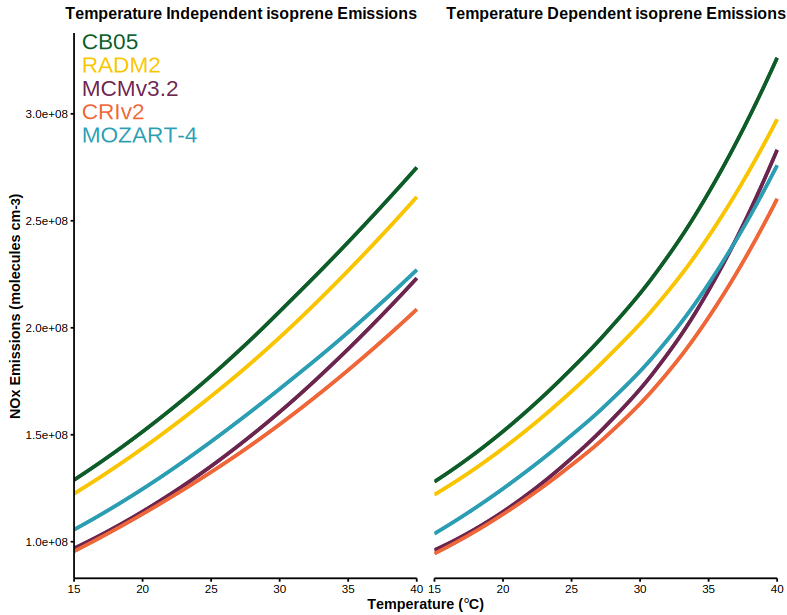
\includegraphics[width = 0.9\textwidth]{img/NOx_emissions_for_Maximal-O3}
\end{figure}

\begin{figure}[ht]
    \centering
    \caption{Contributions to cumulative VOC reactivity (VOCR) from different functional groups of emitted VOCs to the total VOCR. The contributions are normalised by the emissions of each VOC to illustrate the reactivity of each category per molecule emitted. Results illustrated at each temperature, for each chemical mechanism and source of isoprene emissions (temperature-independent and temperature-dependent).}
    \includegraphics[width = 0.9\textwidth]{img/Sum_VOCR_percent_normalised}
\end{figure}

\newpage

\section{Ox Production and Consumption Budgets}
\vspace{-2mm}
Further box model simulations of stagnant conditions were performed as outlined in Section~3.3 of the research article and an analysis similar to that Section~3.2 of the research article looked at the production and consumption budgets of \ce{O_x} was performed.
As in Fig.~4 of the research article the production and consumption of \ce{O_x} are allocated to the net contributions of major categories: `ARO2', `RO2' and `HO2' represent the reaction of acyl peroxy radicals, alkyl peroxy radicals and \ce{HO2} with NO.
`Inorganic' represents the net contribution of inorganic reactions, `RO2NO2' the net contribution of peroxy nitrates and any other reactions were allocated to the `Other Organic' category.
The absolute \ce{O_x} production and consumption budgets for these addition simulations are depicted in Fig.~\ref{f:abs_Ox} while the \ce{O_x} budgets normalised by the total chemical loss rate of emitted VOC are displayed in Fig.~\ref{f:norm_Ox}.
These \ce{O_x} budgets are displayed for each chemical mechanism, \ce{NO_x} condition and source of isoprene emissions (temperature independent and temperature dependent) in Figs.~\ref{f:abs_Ox} and \ref{f:norm_Ox}.
This analysis support the conclusion that the increased OH-reactivity of the emitted VOCs caused the increase of ozone with temperature in our study.
\begin{figure}[ht]
    \centering
    \caption{Day-time budgets of \ce{O_x} from box model simulations without mixing allocated to the \ce{NO_x}-regimes allocated to the net contribution of reactions to \ce{O_x} budgets are allocated to categories of inorganic reactions, peroxy nitrates (RO2NO2), reactions of NO with HO2, alkyl peroxy radicals (RO2) and acyl peroxy radicals (ARO2). All other reactions are allocated to the 'Other Organic' category.}
    \begin{subfigure}[t]{\textwidth}
        \centering
        \caption{Absolute \ce{O_x} production and consumption budgets.}
        \includegraphics[width = 0.97\textwidth]{img/Absolute_Ox_Budget_categories-No_mixing}
        \label{f:abs_Ox}
    \end{subfigure}
    \\
    \begin{subfigure}[t]{\textwidth}
        \centering
        \caption{\ce{O_x} production and consumption budgets normalised by the total chemical loss rate of emitted VOC.}
        \includegraphics[width = 0.97\textwidth]{img/Normalised_Ox_Budget-No_mixing}
        \label{f:norm_Ox}
    \end{subfigure}
\end{figure}

\clearpage
\bibliographystyle{abbrvnat}
\bibliography{References} 

\end{document}
